% Created by tikzDevice version 0.12.6 on 2025-05-12 11:29:37
% !TEX encoding = UTF-8 Unicode
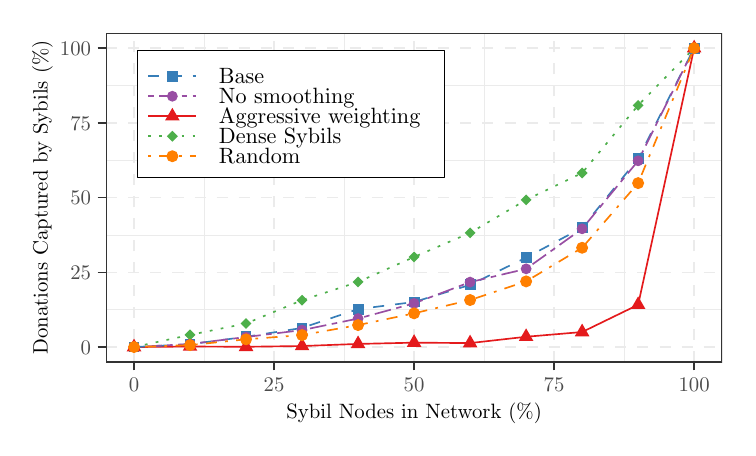
\begin{tikzpicture}[x=1pt,y=1pt]
\definecolor{fillColor}{RGB}{255,255,255}
\path[use as bounding box,fill=fillColor,fill opacity=0.00] (0,0) rectangle (252.94,144.54);
\begin{scope}
\path[clip] (  0.00,  0.00) rectangle (252.94,144.54);
\definecolor{drawColor}{RGB}{255,255,255}
\definecolor{fillColor}{RGB}{255,255,255}

\path[draw=drawColor,line width= 0.6pt,line join=round,line cap=round,fill=fillColor] (  0.00,  0.00) rectangle (252.94,144.54);
\end{scope}
\begin{scope}
\path[clip] ( 28.31, 23.73) rectangle (250.95,142.54);
\definecolor{fillColor}{RGB}{255,255,255}

\path[fill=fillColor] ( 28.31, 23.73) rectangle (250.95,142.54);
\definecolor{drawColor}{gray}{0.92}

\path[draw=drawColor,line width= 0.3pt,line join=round] ( 28.31, 42.63) --
	(250.95, 42.63);

\path[draw=drawColor,line width= 0.3pt,line join=round] ( 28.31, 69.63) --
	(250.95, 69.63);

\path[draw=drawColor,line width= 0.3pt,line join=round] ( 28.31, 96.64) --
	(250.95, 96.64);

\path[draw=drawColor,line width= 0.3pt,line join=round] ( 28.31,123.64) --
	(250.95,123.64);

\path[draw=drawColor,line width= 0.3pt,line join=round] ( 63.73, 23.73) --
	( 63.73,142.54);

\path[draw=drawColor,line width= 0.3pt,line join=round] (114.33, 23.73) --
	(114.33,142.54);

\path[draw=drawColor,line width= 0.3pt,line join=round] (164.93, 23.73) --
	(164.93,142.54);

\path[draw=drawColor,line width= 0.3pt,line join=round] (215.53, 23.73) --
	(215.53,142.54);

\path[draw=drawColor,line width= 0.6pt,dash pattern=on 4pt off 4pt ,line join=round] ( 28.31, 29.13) --
	(250.95, 29.13);

\path[draw=drawColor,line width= 0.6pt,dash pattern=on 4pt off 4pt ,line join=round] ( 28.31, 56.13) --
	(250.95, 56.13);

\path[draw=drawColor,line width= 0.6pt,dash pattern=on 4pt off 4pt ,line join=round] ( 28.31, 83.14) --
	(250.95, 83.14);

\path[draw=drawColor,line width= 0.6pt,dash pattern=on 4pt off 4pt ,line join=round] ( 28.31,110.14) --
	(250.95,110.14);

\path[draw=drawColor,line width= 0.6pt,dash pattern=on 4pt off 4pt ,line join=round] ( 28.31,137.14) --
	(250.95,137.14);

\path[draw=drawColor,line width= 0.6pt,dash pattern=on 4pt off 4pt ,line join=round] ( 38.43, 23.73) --
	( 38.43,142.54);

\path[draw=drawColor,line width= 0.6pt,dash pattern=on 4pt off 4pt ,line join=round] ( 89.03, 23.73) --
	( 89.03,142.54);

\path[draw=drawColor,line width= 0.6pt,dash pattern=on 4pt off 4pt ,line join=round] (139.63, 23.73) --
	(139.63,142.54);

\path[draw=drawColor,line width= 0.6pt,dash pattern=on 4pt off 4pt ,line join=round] (190.23, 23.73) --
	(190.23,142.54);

\path[draw=drawColor,line width= 0.6pt,dash pattern=on 4pt off 4pt ,line join=round] (240.83, 23.73) --
	(240.83,142.54);
\definecolor{drawColor}{RGB}{228,26,28}

\path[draw=drawColor,line width= 0.6pt,line join=round] ( 38.43, 29.13) --
	( 58.67, 29.33) --
	( 78.91, 29.23) --
	( 99.15, 29.50) --
	(119.39, 30.26) --
	(139.63, 30.72) --
	(159.87, 30.57) --
	(180.11, 32.85) --
	(200.35, 34.56) --
	(220.59, 44.41) --
	(240.83,137.14);
\definecolor{drawColor}{RGB}{55,126,184}

\path[draw=drawColor,line width= 0.6pt,dash pattern=on 4pt off 4pt ,line join=round] ( 38.43, 29.13) --
	( 58.67, 30.15) --
	( 78.91, 32.84) --
	( 99.15, 36.04) --
	(119.39, 42.84) --
	(139.63, 45.41) --
	(159.87, 51.60) --
	(180.11, 61.45) --
	(200.35, 72.23) --
	(220.59, 97.20) --
	(240.83,137.14);
\definecolor{drawColor}{RGB}{77,175,74}

\path[draw=drawColor,line width= 0.6pt,dash pattern=on 1pt off 3pt ,line join=round] ( 38.43, 29.13) --
	( 58.67, 33.53) --
	( 78.91, 37.64) --
	( 99.15, 46.07) --
	(119.39, 52.65) --
	(139.63, 61.68) --
	(159.87, 70.40) --
	(180.11, 82.31) --
	(200.35, 92.03) --
	(220.59,116.48) --
	(240.83,137.14);
\definecolor{drawColor}{RGB}{152,78,163}

\path[draw=drawColor,line width= 0.6pt,dash pattern=on 2pt off 2pt on 6pt off 2pt ,line join=round] ( 38.43, 29.13) --
	( 58.67, 30.23) --
	( 78.91, 32.76) --
	( 99.15, 35.25) --
	(119.39, 39.43) --
	(139.63, 44.91) --
	(159.87, 52.60) --
	(180.11, 57.39) --
	(200.35, 71.86) --
	(220.59, 96.43) --
	(240.83,137.14);
\definecolor{drawColor}{RGB}{255,127,0}

\path[draw=drawColor,line width= 0.6pt,dash pattern=on 1pt off 3pt on 4pt off 3pt ,line join=round] ( 38.43, 29.13) --
	( 58.67, 29.84) --
	( 78.91, 31.93) --
	( 99.15, 33.46) --
	(119.39, 37.07) --
	(139.63, 41.32) --
	(159.87, 46.12) --
	(180.11, 52.86) --
	(200.35, 65.00) --
	(220.59, 88.37) --
	(240.83,137.14);
\definecolor{fillColor}{RGB}{55,126,184}

\path[fill=fillColor] ( 36.47, 27.17) --
	( 40.39, 27.17) --
	( 40.39, 31.09) --
	( 36.47, 31.09) --
	cycle;
\definecolor{fillColor}{RGB}{152,78,163}

\path[fill=fillColor] ( 38.43, 29.13) circle (  1.96);
\definecolor{fillColor}{RGB}{228,26,28}

\path[fill=fillColor] ( 38.43, 32.18) --
	( 41.07, 27.60) --
	( 35.79, 27.60) --
	cycle;
\definecolor{fillColor}{RGB}{77,175,74}

\path[fill=fillColor] ( 36.47, 29.13) --
	( 38.43, 31.09) --
	( 40.39, 29.13) --
	( 38.43, 27.17) --
	cycle;
\definecolor{fillColor}{RGB}{255,127,0}

\path[draw=drawColor,line width= 0.4pt,line join=round,line cap=round,fill=fillColor] ( 38.43, 29.13) circle (  1.96);
\definecolor{fillColor}{RGB}{55,126,184}

\path[fill=fillColor] ( 56.71, 28.19) --
	( 60.63, 28.19) --
	( 60.63, 32.12) --
	( 56.71, 32.12) --
	cycle;
\definecolor{fillColor}{RGB}{152,78,163}

\path[fill=fillColor] ( 58.67, 30.23) circle (  1.96);
\definecolor{fillColor}{RGB}{228,26,28}

\path[fill=fillColor] ( 58.67, 32.38) --
	( 61.31, 27.80) --
	( 56.03, 27.80) --
	cycle;
\definecolor{fillColor}{RGB}{77,175,74}

\path[fill=fillColor] ( 56.71, 33.53) --
	( 58.67, 35.49) --
	( 60.63, 33.53) --
	( 58.67, 31.57) --
	cycle;
\definecolor{fillColor}{RGB}{255,127,0}

\path[draw=drawColor,line width= 0.4pt,line join=round,line cap=round,fill=fillColor] ( 58.67, 29.84) circle (  1.96);
\definecolor{fillColor}{RGB}{55,126,184}

\path[fill=fillColor] ( 76.95, 30.88) --
	( 80.87, 30.88) --
	( 80.87, 34.80) --
	( 76.95, 34.80) --
	cycle;
\definecolor{fillColor}{RGB}{152,78,163}

\path[fill=fillColor] ( 78.91, 32.76) circle (  1.96);
\definecolor{fillColor}{RGB}{228,26,28}

\path[fill=fillColor] ( 78.91, 32.28) --
	( 81.55, 27.70) --
	( 76.27, 27.70) --
	cycle;
\definecolor{fillColor}{RGB}{77,175,74}

\path[fill=fillColor] ( 76.95, 37.64) --
	( 78.91, 39.60) --
	( 80.87, 37.64) --
	( 78.91, 35.68) --
	cycle;
\definecolor{fillColor}{RGB}{255,127,0}

\path[draw=drawColor,line width= 0.4pt,line join=round,line cap=round,fill=fillColor] ( 78.91, 31.93) circle (  1.96);
\definecolor{fillColor}{RGB}{55,126,184}

\path[fill=fillColor] ( 97.19, 34.08) --
	(101.11, 34.08) --
	(101.11, 38.00) --
	( 97.19, 38.00) --
	cycle;
\definecolor{fillColor}{RGB}{152,78,163}

\path[fill=fillColor] ( 99.15, 35.25) circle (  1.96);
\definecolor{fillColor}{RGB}{228,26,28}

\path[fill=fillColor] ( 99.15, 32.55) --
	(101.79, 27.98) --
	( 96.51, 27.98) --
	cycle;
\definecolor{fillColor}{RGB}{77,175,74}

\path[fill=fillColor] ( 97.19, 46.07) --
	( 99.15, 48.03) --
	(101.11, 46.07) --
	( 99.15, 44.10) --
	cycle;
\definecolor{fillColor}{RGB}{255,127,0}

\path[draw=drawColor,line width= 0.4pt,line join=round,line cap=round,fill=fillColor] ( 99.15, 33.46) circle (  1.96);
\definecolor{fillColor}{RGB}{55,126,184}

\path[fill=fillColor] (117.43, 40.88) --
	(121.35, 40.88) --
	(121.35, 44.81) --
	(117.43, 44.81) --
	cycle;
\definecolor{fillColor}{RGB}{152,78,163}

\path[fill=fillColor] (119.39, 39.43) circle (  1.96);
\definecolor{fillColor}{RGB}{228,26,28}

\path[fill=fillColor] (119.39, 33.31) --
	(122.03, 28.74) --
	(116.75, 28.74) --
	cycle;
\definecolor{fillColor}{RGB}{77,175,74}

\path[fill=fillColor] (117.43, 52.65) --
	(119.39, 54.61) --
	(121.35, 52.65) --
	(119.39, 50.68) --
	cycle;
\definecolor{fillColor}{RGB}{255,127,0}

\path[draw=drawColor,line width= 0.4pt,line join=round,line cap=round,fill=fillColor] (119.39, 37.07) circle (  1.96);
\definecolor{fillColor}{RGB}{55,126,184}

\path[fill=fillColor] (137.67, 43.45) --
	(141.59, 43.45) --
	(141.59, 47.38) --
	(137.67, 47.38) --
	cycle;
\definecolor{fillColor}{RGB}{152,78,163}

\path[fill=fillColor] (139.63, 44.91) circle (  1.96);
\definecolor{fillColor}{RGB}{228,26,28}

\path[fill=fillColor] (139.63, 33.77) --
	(142.27, 29.20) --
	(136.99, 29.20) --
	cycle;
\definecolor{fillColor}{RGB}{77,175,74}

\path[fill=fillColor] (137.67, 61.68) --
	(139.63, 63.64) --
	(141.59, 61.68) --
	(139.63, 59.72) --
	cycle;
\definecolor{fillColor}{RGB}{255,127,0}

\path[draw=drawColor,line width= 0.4pt,line join=round,line cap=round,fill=fillColor] (139.63, 41.32) circle (  1.96);
\definecolor{fillColor}{RGB}{55,126,184}

\path[fill=fillColor] (157.91, 49.64) --
	(161.83, 49.64) --
	(161.83, 53.57) --
	(157.91, 53.57) --
	cycle;
\definecolor{fillColor}{RGB}{152,78,163}

\path[fill=fillColor] (159.87, 52.60) circle (  1.96);
\definecolor{fillColor}{RGB}{228,26,28}

\path[fill=fillColor] (159.87, 33.62) --
	(162.51, 29.04) --
	(157.23, 29.04) --
	cycle;
\definecolor{fillColor}{RGB}{77,175,74}

\path[fill=fillColor] (157.91, 70.40) --
	(159.87, 72.36) --
	(161.83, 70.40) --
	(159.87, 68.44) --
	cycle;
\definecolor{fillColor}{RGB}{255,127,0}

\path[draw=drawColor,line width= 0.4pt,line join=round,line cap=round,fill=fillColor] (159.87, 46.12) circle (  1.96);
\definecolor{fillColor}{RGB}{55,126,184}

\path[fill=fillColor] (178.15, 59.49) --
	(182.07, 59.49) --
	(182.07, 63.42) --
	(178.15, 63.42) --
	cycle;
\definecolor{fillColor}{RGB}{152,78,163}

\path[fill=fillColor] (180.11, 57.39) circle (  1.96);
\definecolor{fillColor}{RGB}{228,26,28}

\path[fill=fillColor] (180.11, 35.90) --
	(182.75, 31.33) --
	(177.46, 31.33) --
	cycle;
\definecolor{fillColor}{RGB}{77,175,74}

\path[fill=fillColor] (178.15, 82.31) --
	(180.11, 84.27) --
	(182.07, 82.31) --
	(180.11, 80.35) --
	cycle;
\definecolor{fillColor}{RGB}{255,127,0}

\path[draw=drawColor,line width= 0.4pt,line join=round,line cap=round,fill=fillColor] (180.11, 52.86) circle (  1.96);
\definecolor{fillColor}{RGB}{55,126,184}

\path[fill=fillColor] (198.38, 70.27) --
	(202.31, 70.27) --
	(202.31, 74.19) --
	(198.38, 74.19) --
	cycle;
\definecolor{fillColor}{RGB}{152,78,163}

\path[fill=fillColor] (200.35, 71.86) circle (  1.96);
\definecolor{fillColor}{RGB}{228,26,28}

\path[fill=fillColor] (200.35, 37.61) --
	(202.99, 33.03) --
	(197.70, 33.03) --
	cycle;
\definecolor{fillColor}{RGB}{77,175,74}

\path[fill=fillColor] (198.38, 92.03) --
	(200.35, 93.99) --
	(202.31, 92.03) --
	(200.35, 90.07) --
	cycle;
\definecolor{fillColor}{RGB}{255,127,0}

\path[draw=drawColor,line width= 0.4pt,line join=round,line cap=round,fill=fillColor] (200.35, 65.00) circle (  1.96);
\definecolor{fillColor}{RGB}{55,126,184}

\path[fill=fillColor] (218.62, 95.24) --
	(222.55, 95.24) --
	(222.55, 99.16) --
	(218.62, 99.16) --
	cycle;
\definecolor{fillColor}{RGB}{152,78,163}

\path[fill=fillColor] (220.59, 96.43) circle (  1.96);
\definecolor{fillColor}{RGB}{228,26,28}

\path[fill=fillColor] (220.59, 47.46) --
	(223.23, 42.89) --
	(217.94, 42.89) --
	cycle;
\definecolor{fillColor}{RGB}{77,175,74}

\path[fill=fillColor] (218.62,116.48) --
	(220.59,118.44) --
	(222.55,116.48) --
	(220.59,114.52) --
	cycle;
\definecolor{fillColor}{RGB}{255,127,0}

\path[draw=drawColor,line width= 0.4pt,line join=round,line cap=round,fill=fillColor] (220.59, 88.37) circle (  1.96);
\definecolor{fillColor}{RGB}{55,126,184}

\path[fill=fillColor] (238.86,135.18) --
	(242.79,135.18) --
	(242.79,139.10) --
	(238.86,139.10) --
	cycle;
\definecolor{fillColor}{RGB}{152,78,163}

\path[fill=fillColor] (240.83,137.14) circle (  1.96);
\definecolor{fillColor}{RGB}{228,26,28}

\path[fill=fillColor] (240.83,140.19) --
	(243.47,135.61) --
	(238.18,135.61) --
	cycle;
\definecolor{fillColor}{RGB}{77,175,74}

\path[fill=fillColor] (238.86,137.14) --
	(240.83,139.10) --
	(242.79,137.14) --
	(240.83,135.18) --
	cycle;
\definecolor{fillColor}{RGB}{255,127,0}

\path[draw=drawColor,line width= 0.4pt,line join=round,line cap=round,fill=fillColor] (240.83,137.14) circle (  1.96);
\definecolor{drawColor}{gray}{0.20}

\path[draw=drawColor,line width= 0.6pt,line join=round,line cap=round] ( 28.31, 23.73) rectangle (250.95,142.54);
\end{scope}
\begin{scope}
\path[clip] (  0.00,  0.00) rectangle (252.94,144.54);
\definecolor{drawColor}{gray}{0.30}

\node[text=drawColor,anchor=base east,inner sep=0pt, outer sep=0pt, scale=  0.75] at ( 22.91, 26.53) {0};

\node[text=drawColor,anchor=base east,inner sep=0pt, outer sep=0pt, scale=  0.75] at ( 22.91, 53.53) {25};

\node[text=drawColor,anchor=base east,inner sep=0pt, outer sep=0pt, scale=  0.75] at ( 22.91, 80.53) {50};

\node[text=drawColor,anchor=base east,inner sep=0pt, outer sep=0pt, scale=  0.75] at ( 22.91,107.53) {75};

\node[text=drawColor,anchor=base east,inner sep=0pt, outer sep=0pt, scale=  0.75] at ( 22.91,134.54) {100};
\end{scope}
\begin{scope}
\path[clip] (  0.00,  0.00) rectangle (252.94,144.54);
\definecolor{drawColor}{gray}{0.20}

\path[draw=drawColor,line width= 0.6pt,line join=round] ( 25.31, 29.13) --
	( 28.31, 29.13);

\path[draw=drawColor,line width= 0.6pt,line join=round] ( 25.31, 56.13) --
	( 28.31, 56.13);

\path[draw=drawColor,line width= 0.6pt,line join=round] ( 25.31, 83.14) --
	( 28.31, 83.14);

\path[draw=drawColor,line width= 0.6pt,line join=round] ( 25.31,110.14) --
	( 28.31,110.14);

\path[draw=drawColor,line width= 0.6pt,line join=round] ( 25.31,137.14) --
	( 28.31,137.14);
\end{scope}
\begin{scope}
\path[clip] (  0.00,  0.00) rectangle (252.94,144.54);
\definecolor{drawColor}{gray}{0.20}

\path[draw=drawColor,line width= 0.6pt,line join=round] ( 38.43, 20.73) --
	( 38.43, 23.73);

\path[draw=drawColor,line width= 0.6pt,line join=round] ( 89.03, 20.73) --
	( 89.03, 23.73);

\path[draw=drawColor,line width= 0.6pt,line join=round] (139.63, 20.73) --
	(139.63, 23.73);

\path[draw=drawColor,line width= 0.6pt,line join=round] (190.23, 20.73) --
	(190.23, 23.73);

\path[draw=drawColor,line width= 0.6pt,line join=round] (240.83, 20.73) --
	(240.83, 23.73);
\end{scope}
\begin{scope}
\path[clip] (  0.00,  0.00) rectangle (252.94,144.54);
\definecolor{drawColor}{gray}{0.30}

\node[text=drawColor,anchor=base,inner sep=0pt, outer sep=0pt, scale=  0.75] at ( 38.43, 13.12) {0};

\node[text=drawColor,anchor=base,inner sep=0pt, outer sep=0pt, scale=  0.75] at ( 89.03, 13.12) {25};

\node[text=drawColor,anchor=base,inner sep=0pt, outer sep=0pt, scale=  0.75] at (139.63, 13.12) {50};

\node[text=drawColor,anchor=base,inner sep=0pt, outer sep=0pt, scale=  0.75] at (190.23, 13.12) {75};

\node[text=drawColor,anchor=base,inner sep=0pt, outer sep=0pt, scale=  0.75] at (240.83, 13.12) {100};
\end{scope}
\begin{scope}
\path[clip] (  0.00,  0.00) rectangle (252.94,144.54);
\definecolor{drawColor}{RGB}{0,0,0}

\node[text=drawColor,anchor=base,inner sep=0pt, outer sep=0pt, scale=  0.75] at (139.63,  3.46) {Sybil Nodes in Network ({\%})};
\end{scope}
\begin{scope}
\path[clip] (  0.00,  0.00) rectangle (252.94,144.54);
\definecolor{drawColor}{RGB}{0,0,0}

\node[text=drawColor,rotate= 90.00,anchor=base,inner sep=0pt, outer sep=0pt, scale=  0.75] at (  7.21, 83.14) {Donations Captured by Sybils ({\%})};
\end{scope}
\begin{scope}
\path[clip] (  0.00,  0.00) rectangle (252.94,144.54);
\definecolor{drawColor}{RGB}{0,0,0}
\definecolor{fillColor}{RGB}{255,255,255}

\path[draw=drawColor,line width= 0.1pt,line join=round,line cap=round,fill=fillColor] ( 39.44, 90.46) rectangle (150.46,136.60);
\end{scope}
\begin{scope}
\path[clip] (  0.00,  0.00) rectangle (252.94,144.54);
\definecolor{fillColor}{RGB}{255,255,255}

\path[fill=fillColor] ( 41.44,123.37) rectangle ( 63.12,130.60);
\end{scope}
\begin{scope}
\path[clip] (  0.00,  0.00) rectangle (252.94,144.54);
\definecolor{drawColor}{RGB}{55,126,184}

\path[draw=drawColor,line width= 0.6pt,dash pattern=on 4pt off 4pt ,line join=round] ( 43.61,126.99) -- ( 60.96,126.99);
\end{scope}
\begin{scope}
\path[clip] (  0.00,  0.00) rectangle (252.94,144.54);
\definecolor{fillColor}{RGB}{55,126,184}

\path[fill=fillColor] ( 50.32,125.02) --
	( 54.25,125.02) --
	( 54.25,128.95) --
	( 50.32,128.95) --
	cycle;
\end{scope}
\begin{scope}
\path[clip] (  0.00,  0.00) rectangle (252.94,144.54);
\definecolor{fillColor}{RGB}{255,255,255}

\path[fill=fillColor] ( 41.44,116.15) rectangle ( 63.12,123.37);
\end{scope}
\begin{scope}
\path[clip] (  0.00,  0.00) rectangle (252.94,144.54);
\definecolor{drawColor}{RGB}{152,78,163}

\path[draw=drawColor,line width= 0.6pt,dash pattern=on 2pt off 2pt on 6pt off 2pt ,line join=round] ( 43.61,119.76) -- ( 60.96,119.76);
\end{scope}
\begin{scope}
\path[clip] (  0.00,  0.00) rectangle (252.94,144.54);
\definecolor{fillColor}{RGB}{152,78,163}

\path[fill=fillColor] ( 52.28,119.76) circle (  1.96);
\end{scope}
\begin{scope}
\path[clip] (  0.00,  0.00) rectangle (252.94,144.54);
\definecolor{fillColor}{RGB}{255,255,255}

\path[fill=fillColor] ( 41.44,108.92) rectangle ( 63.12,116.15);
\end{scope}
\begin{scope}
\path[clip] (  0.00,  0.00) rectangle (252.94,144.54);
\definecolor{drawColor}{RGB}{228,26,28}

\path[draw=drawColor,line width= 0.6pt,line join=round] ( 43.61,112.53) -- ( 60.96,112.53);
\end{scope}
\begin{scope}
\path[clip] (  0.00,  0.00) rectangle (252.94,144.54);
\definecolor{fillColor}{RGB}{228,26,28}

\path[fill=fillColor] ( 52.28,115.58) --
	( 54.93,111.01) --
	( 49.64,111.01) --
	cycle;
\end{scope}
\begin{scope}
\path[clip] (  0.00,  0.00) rectangle (252.94,144.54);
\definecolor{fillColor}{RGB}{255,255,255}

\path[fill=fillColor] ( 41.44,101.69) rectangle ( 63.12,108.92);
\end{scope}
\begin{scope}
\path[clip] (  0.00,  0.00) rectangle (252.94,144.54);
\definecolor{drawColor}{RGB}{77,175,74}

\path[draw=drawColor,line width= 0.6pt,dash pattern=on 1pt off 3pt ,line join=round] ( 43.61,105.31) -- ( 60.96,105.31);
\end{scope}
\begin{scope}
\path[clip] (  0.00,  0.00) rectangle (252.94,144.54);
\definecolor{fillColor}{RGB}{77,175,74}

\path[fill=fillColor] ( 50.32,105.31) --
	( 52.28,107.27) --
	( 54.25,105.31) --
	( 52.28,103.34) --
	cycle;
\end{scope}
\begin{scope}
\path[clip] (  0.00,  0.00) rectangle (252.94,144.54);
\definecolor{fillColor}{RGB}{255,255,255}

\path[fill=fillColor] ( 41.44, 94.46) rectangle ( 63.12,101.69);
\end{scope}
\begin{scope}
\path[clip] (  0.00,  0.00) rectangle (252.94,144.54);
\definecolor{drawColor}{RGB}{255,127,0}

\path[draw=drawColor,line width= 0.6pt,dash pattern=on 1pt off 3pt on 4pt off 3pt ,line join=round] ( 43.61, 98.08) -- ( 60.96, 98.08);
\end{scope}
\begin{scope}
\path[clip] (  0.00,  0.00) rectangle (252.94,144.54);
\definecolor{drawColor}{RGB}{255,127,0}
\definecolor{fillColor}{RGB}{255,127,0}

\path[draw=drawColor,line width= 0.4pt,line join=round,line cap=round,fill=fillColor] ( 52.28, 98.08) circle (  1.96);
\end{scope}
\begin{scope}
\path[clip] (  0.00,  0.00) rectangle (252.94,144.54);
\definecolor{drawColor}{RGB}{0,0,0}

\node[text=drawColor,anchor=base west,inner sep=0pt, outer sep=0pt, scale=  0.80] at ( 69.12,124.21) {Base};
\end{scope}
\begin{scope}
\path[clip] (  0.00,  0.00) rectangle (252.94,144.54);
\definecolor{drawColor}{RGB}{0,0,0}

\node[text=drawColor,anchor=base west,inner sep=0pt, outer sep=0pt, scale=  0.80] at ( 69.12,116.98) {No smoothing};
\end{scope}
\begin{scope}
\path[clip] (  0.00,  0.00) rectangle (252.94,144.54);
\definecolor{drawColor}{RGB}{0,0,0}

\node[text=drawColor,anchor=base west,inner sep=0pt, outer sep=0pt, scale=  0.80] at ( 69.12,109.75) {Aggressive weighting};
\end{scope}
\begin{scope}
\path[clip] (  0.00,  0.00) rectangle (252.94,144.54);
\definecolor{drawColor}{RGB}{0,0,0}

\node[text=drawColor,anchor=base west,inner sep=0pt, outer sep=0pt, scale=  0.80] at ( 69.12,102.53) {Dense Sybils};
\end{scope}
\begin{scope}
\path[clip] (  0.00,  0.00) rectangle (252.94,144.54);
\definecolor{drawColor}{RGB}{0,0,0}

\node[text=drawColor,anchor=base west,inner sep=0pt, outer sep=0pt, scale=  0.80] at ( 69.12, 95.30) {Random};
\end{scope}
\end{tikzpicture}
